%%
% Please see https://bitbucket.org/rivanvx/beamer/wiki/Home for obtaining beamer.
%%
\documentclass[aspectratio=169]{beamer}
\usetheme{Antibes}
\usepackage{xcolor}
\mode<presentation>

\useoutertheme{miniframes} 
\useinnertheme{circles}

\definecolor{primary}{HTML}{003469}
\definecolor{secondary}{HTML}{003469}
\definecolor{tertiary}{HTML}{00addc}


\setbeamercolor{titlelike}{bg=white,fg=primary}

\setbeamercolor{palette primary}{bg=tertiary,fg=white}
\setbeamercolor{palette secondary}{bg=tertiary,fg=white}
\setbeamercolor{palette tertiary}{bg=secondary,fg=white}
\setbeamercolor{structure}{fg=secondary} % itemize, enumerate, etc
\setbeamercolor{section in toc}{fg=secondary} % TOC sections
% Override palette coloring with secondary
\setbeamercolor{subsection in head/foot}{bg=tertiary,fg=white}
\usepackage{natbib}
\bibliographystyle{unsrtnat}
\setcitestyle{authoryear,open={(},close={)}}
\usepackage{csquotes}
\usepackage{hyperref}

\hypersetup{
    colorlinks=true,
    linkcolor=black,
    filecolor=black,      
    urlcolor=cyan,
    pdftitle={Python, Cloud and Automation for TE: 2. Getting Started},
    }



\title{\large{\textbf{Python, Cloud and Automation}} \newline\newline 2. Getting Started with Python}

\author{Jack Minchin}
\institute{Tourism Economics}
\date{2022}

\begin{document}

\frame{\titlepage}

\begin{frame}
\frametitle{Table of Contents}
\tableofcontents
\end{frame}

\section{Downloading}
\begin{frame}{Downloading Python}

\begin{itemize}
	\item Python can be downloaded from its official website:
\href{https://www.python.org/downloads/release/python-3104/}{Download here}

\item Python is not a programme, so you won't see any new programmes to run, or any editor to write code in. When you install Python, you are installing a set of instructions that tells your computer how to interpret and run python code. 

\end{itemize}

	
\end{frame}



\section{Basic Concepts}

\begin{frame}{Editing Code}
\begin{columns}

\begin{column}{0.4\textwidth}
\begin{enumerate}
  \item Coding is writing text files, theoretically this can be done in TextEdit or Notepad but there are far better tools to help write code. 
	
	\item The most populate code editor is \href{https://code.visualstudio.com}{VS Code}, it has features such as syntax highlighting, autocomplete, documentation and an integrated terminal. 
\end{enumerate}

\end{column}

\begin{column}{0.6\textwidth}
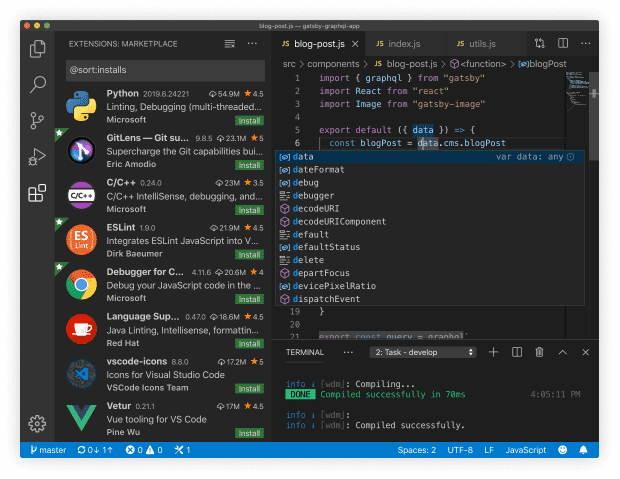
\includegraphics[width=0.9\linewidth]{graphics/home-screenshot-mac.png}	
\end{column}


\end{columns}

	
	
		
\end{frame}


\begin{frame}{Writing in python}
	\begin{itemize}
		\item \textbf{.py files}
		
		The most basic Python file is the .py file, this is just a text file with the .py extension. Python files (generally) run end-to-end without stopping and without providing output. 
		
		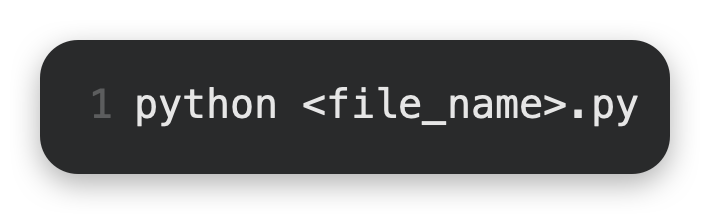
\includegraphics[scale=0.5]{graphics/run_python_file.png}
		
		These are best suited for when you have larger applications, with interlinking modules or tasks that run repetitively that don't require manual checks at each step. 
			
	\end{itemize}
\end{frame}


\begin{frame}{Writing in python}
	\begin{columns}
	
	\begin{column}{0.6\textwidth}
	
		\textbf{Python Notebooks}
		
		\begin{itemize}	

		\item Python notebooks are files that end in .ipynb, and provide an easier way to write python code and explore the outputs, creating editable and shareable files. 
		\item Notebooks are structured in code cells, which can be run independently of one another with the output of the cell displayed underneath.
	\end{itemize}
		
	\end{column}
	
		\begin{column}{0.4\textwidth}
		
		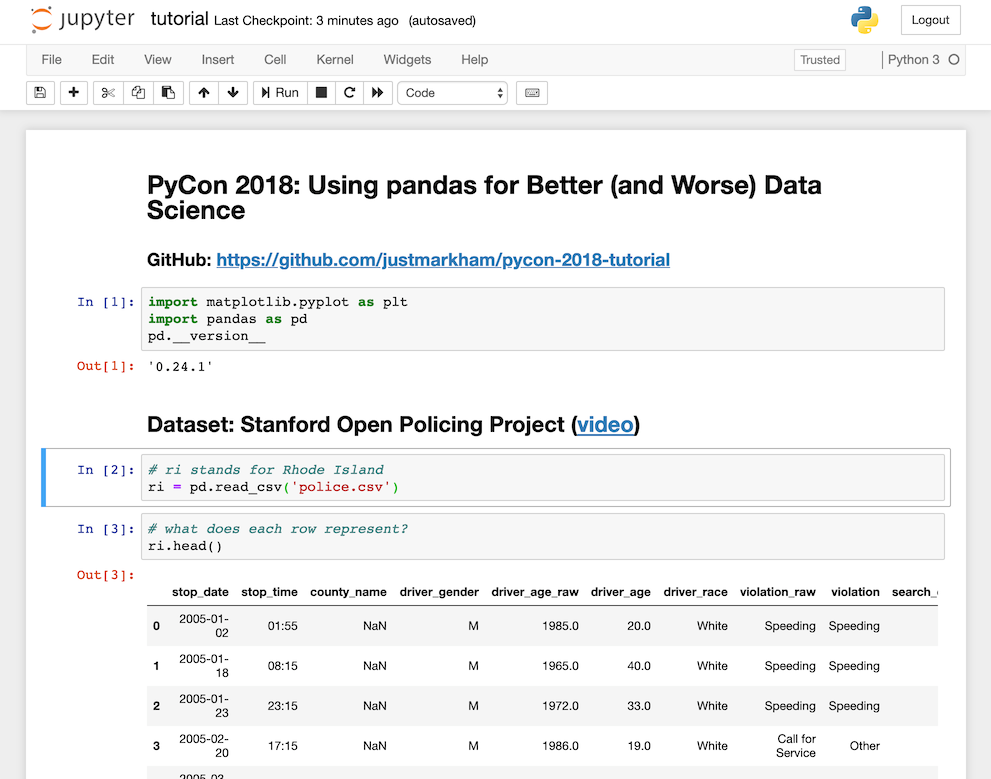
\includegraphics[scale=.6]{graphics/notebook.png}
			
	\end{column}
	\end{columns}
\end{frame}

\section{Environments}


\begin{frame}{Virtual environments}

\begin{itemize}
	\item A virtual environment is a Python environment such that the Python interpreter, libraries and scripts installed into it are isolated from those installed in other virtual environments, and (by default) any libraries installed in a “system” Python, i.e., one which is installed as part of your operating system.
	\item When writing code, you will more than likely be using module written by other organisations and users, over time your main python environment (the one we installed at the start) will get cluttered, therefore it is useful to have a separate virtual environment for each project. 
\end{itemize}
 	
\end{frame}

\section{Managing Projects}

\begin{frame}{Managing Projects: Git}


	\begin{itemize}
		\item Code projects are changed and updated often, particularly when they are worked on by multiple people. 
		\item When creating a new version or an update, the code is not copied into a new directory but the same directory is used and Git is used to manage versioning.
		\item Git uses commits and branches which can be merged together to allow multiple people to work on one code base and ensure that there are no conflicts. 
	\end{itemize}

\begin{figure}
\centering	
	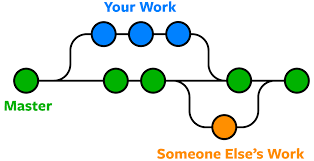
\includegraphics[scale=0.5]{graphics/git.png}
\end{figure}

\end{frame}

\begin{frame}{Git continued}

\begin{itemize}
	\item Git is not just for Python it is used for all coding languages and even projects that aren't code. For example, the directory that holds these slides is managed by git.
	\item Git repositories, while stored in your computer are also synced over the internet, they can be private or public.
	\item It is not similar to OneDrive however, in order to sync someones changes, you must manually 'pull' the changes and in order to 'push' to the repository you must merge branches manually. 
	\item Git repositories also ease the process of deploying code and solutions to cloud providers. 
\end{itemize}


\end{frame}

\end{frame




\end{document}
